\chapter{Анализ методов синтеза регулярных нелинейных узлов замен}

Основным и наиболее  эффективным механизмом криптографической защиты информации
являются методы блочного симметричного криптографического преобразования.
Наряду с высокой скоростью преобразований и простотой практической реализации
симметричные криптоалгоритмы позволяют обеспечить высокую стойкость к различным
методам криптографического анализа.

Основным элементом современных блочных симметричных криптографических средств
защиты информации являются нелинейные узлы замен (нелинейные блоки подстановок),
качество построения которых непосредственновлияет на эффективность
разрабатываемых механизмов обеспечения безопасности информационных технологий.

На сегодняшний день в Украине нет национального алгоритма блочного симметричного
криптографического преобразования информации. Правила формирования нелинейных
узлов замен ныне действующего стандарта ГОСТ 28147-89 являются государственной
тайной Российской Федерации и не доступны для использования в Украине. В этом
смысле разработка математической модели и вычислительного метода формирования
нелинейных узлов замен с  высокими показателями стойкости является актуальной
научно-технической задачей, непосредственно связанной с выполнением ряда важных
государственных программ Украины и проводимым в недавнее время открытым
конкурсом симметричных криптографических алгоритмов.

Нелинейные узлы замен блочных  симметричных криптографических средств защиты
информации эффективно описываются в математическом виде совокупностью
криптографических булевых функций и накладываемой системой ограничений на
отдельные показатели стойкости. Таким образом, использование математического
аппарата булевой алгебры позволяет получить абстрактное аналитическое описание
нелинейных узлов замен и адекватно оценивать их стойкость.

В данном разделе исследуется структура и основные функциональные элементы
алгоритмов блочного симметричного криптографического преобразования информации,
обосновываются требования к перспективным методам блочного симметричного
криптографического преобразования, исследуется математический аппарат булевой
алгебры для построения нелинейных узлов замен  блочных симметричных
криптопреобразований, проводится анализ различных подходов к построению
нелинейных узлов замен, исследуются основные показатели стойкости нелинейных
узлов замен современных блочных симметричных шифров.

\section{Сравнительный анализ методов блочного симметричного криптографического
преобразования информации}

Для защиты информации с ограниченным доступом в современных информационных
системах применяются различные криптографические средства. Основным и наиболее
эффективным механизмом криптографической защиты информации являются методы
блочного симметричного криптографического преобразования. Наряду с высокой
скоростью преобразований и  простотой практической реализации симметричные
криптоалгоритмы позволяют обеспечить высокую стойкость к различным методам
криптографического анализа. Проведем анализ и сравнительное исследование методов
блочного симметричного  криптографического преобразования информации.

Как показывает анализ открытой литературы и результаты проводимых
криптографических конкурсов, на сегодняшний день реализовано большое число
различных блочных симметричных методов преобразования информации. При этом
подавляющее большинство методов делится на две большие группы: 

\begin{itemize}

    \item методы, построенные на основе использования цепей Фейстеля;

    \item методы, построенные на основе чередования процедур перестановок и
    подстановок, т.н. SP-конструкций. 

\end{itemize}

Приведём основные определения и обозначения блочных симметричных шифров и схем
их построения.

Пусть $T$ и $K$ "--- пространства текстов и ключей соответственно блочного
симметричного шифра.
\begin{equation}C = \{C_k: T \rightarrow T: k \in K\}\end{equation}

Пусть $r > 0$ "--- положительное целое и пусть $K_1, K_2, \ldots, K_r$ "--- $r$
конечных множеств. Говорят, что $C$ "--- $r$-раундовый итеративный блочный
симметричный шифр (БСШ), если он может быть записан в виде:
\begin{equation}C_k = R^{(r)}_{k_r} \circ R^{(r-1)}_{k_{r-1}} \circ \ldots \circ
R^{1}_{k_1}\end{equation}

для всех $k \in K$, где
\begin{equation}R^{(i)} = \{R^{(i)}_{k_i}: T \rightarrow T: k_i \in
K_i\}\end{equation}

называется $i$-м раундом $С$. 

Обычно $i$-й раунд блочного симметричного шифра состоит из трех слоев: слоя
подстановочного преобразования с использованием нелинейных блоков замен или
S-блоков,  слоя линейного перестановочного преобразования и  слоя функциональных
преобразований, таких как сдвиг, сложение по модулю с ключом и пр.

Такой итеративный подстановочно-перестановочный подход к разработке стойких
симметричных шифров был основан К. Шенноном и использует два общих принципа
построения: перемешивание (confusion) и рассеивание (diffusion). Перемешивание
осуществляет распространение влияния одного знака открытого текста на множество
символов шифртекста, что обуславливает лавинный эффект (в случае блочных шифров
"--- обеспечение распространения влияния каждого бита входного текста на все
биты выходного текста). Рассеиванием называется шифрующее преобразование,
нарушающее взаимосвязи статистических характеристик входного и выходного текста,
т.е. маскировку статистических свойств исходного сообщения.

Ключи $k_1, k_2, \ldots, k_r$ называются раундовыми ключами блочного
симметричного шифра и производятся из одного основного секретного ключа $k$
посредством детерминистического алгоритма, называемого алгоритмом распределения
ключей.

Схема Фейстеля (см. рис.~\ref{fig:feistel}) является структурой, которая
позволяет построить перестановку для $2n$-битных последовательностей,
основываясь на функциях от $n$-битных последовательностей. Обозначим схему
Фейстеля с $r > 0$ раундами преобразования, основанных на функциях
$f_1, f_2, \ldots, f_r: \{0, 1\}^n \rightarrow \{0, 1\}^n$

как $\Phi(f_1, f_2, \ldots, f_r)$. Легко заметить, что $\Phi(f_1, f_2, \ldots, f_r)$
обратима, т.к.
\begin{equation}\Phi^{-1}(f_1, f_2, \ldots, f_r) = \Phi(f_r, f_{r-1}, \ldots, f_1)\end{equation}

\begin{figure}
    \centering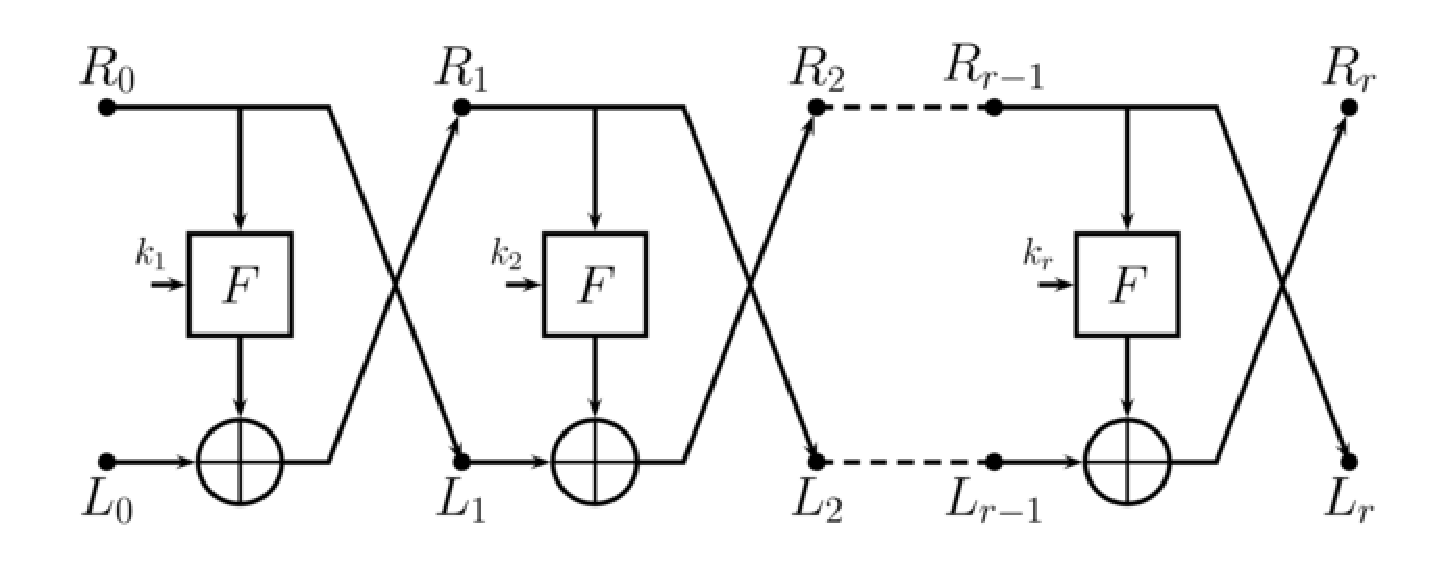
\includegraphics[width=1\textwidth]{feistel.eps}
    \caption{$r$–раундовая схема Фейстеля $\Phi(f_1, f_2, \ldots, f_r)$}
    \label{fig:feistel}
\end{figure}

Подстановочно-перестановочная структура (SP-структура, Substitution Permutation)
наиболее близка к принципам построения К. Шеннона и состоит из
последовательности слоев, в которых подстановочный слой осуществляет
перемешивание, за которым следует перестановочный слой, осуществляющий
рассеивание. SP-схема проиллюстрирована на рисунке~\ref{fig:SP}.

Все преобразования в SP-конструкциях должны быть обратимыми, так как
расшифрование производится путем выполнения обратных преобразований в обратном
порядке.

Оба вида  конструкций имеют свои достоинства и недостатки. Так, преимуществом
конструкции Фейстеля в сравнении с SP-конструкцией является значительное
облегчение практической реализации на процессорах малой разрядности, поскольку
обрабатываемые итеративной процедурой данные разбиваются на 2 блока и обработка
криптопримитивами производится над подблоками. Другим преимуществом является то,
что конструкция Фейстеля позволяет использовать в шифрующей функции более
широкий набор преобразований, так как к ним не предъявляется требование
обратимости.

\begin{figure}
    \centering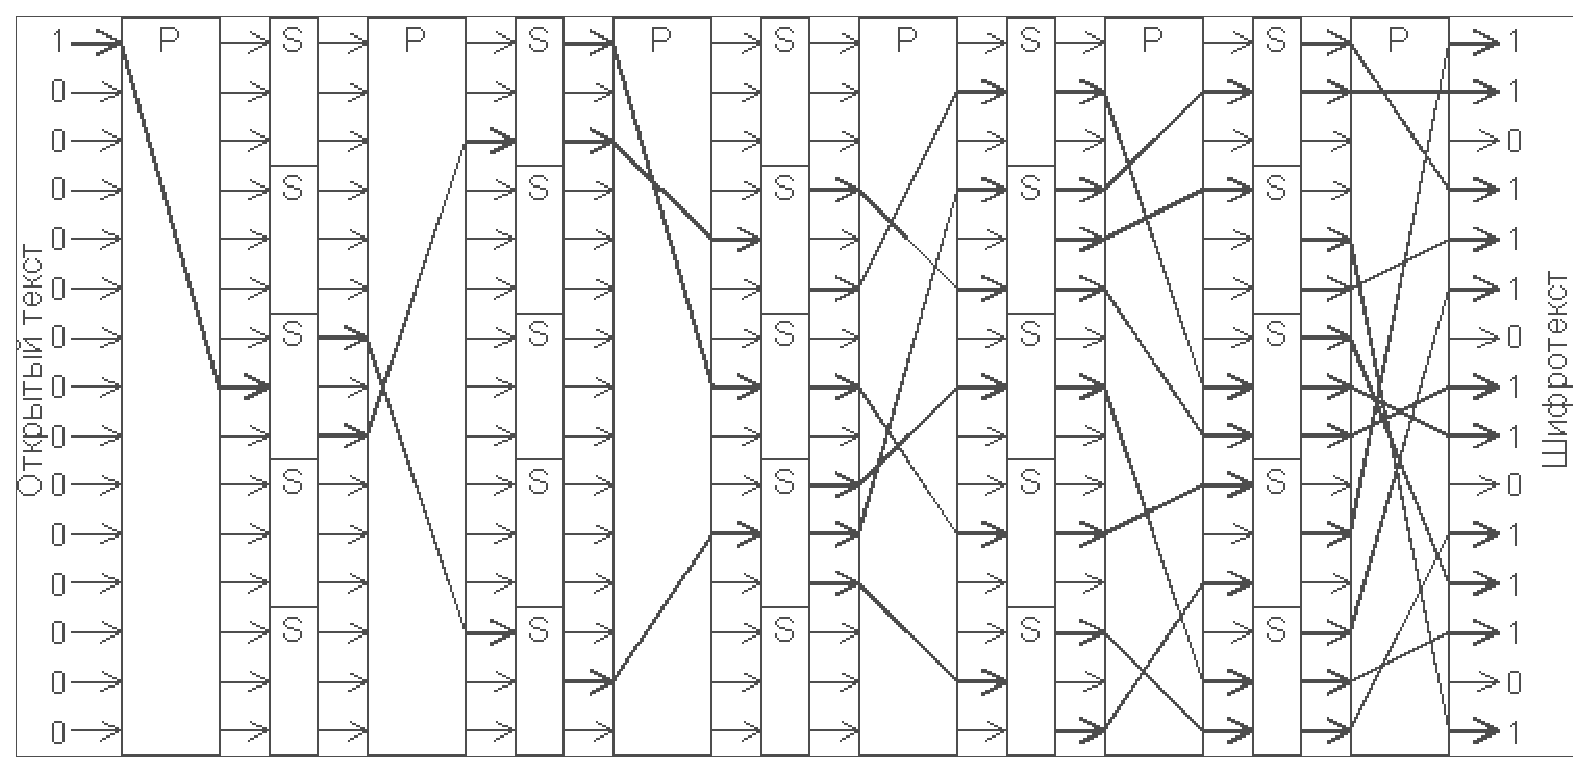
\includegraphics[width=1\textwidth]{sp.eps}
    \caption{SP-схема}
    \label{fig:SP}
\end{figure}

В то же время блоки подстановок и перестановок, применяемые в конструкциях
Фейстеля, имеют небольшой размер. Размерность же блоков нелинейного
подстановочного и линейного перестановочного преобразования в SP-конструкциях
значительно больше, что приводит к усилению устойчивости к различным методам
криптоанализа. Другим преимуществом SP структуры является ее большая
прозрачность и приближенность к принципам построения стойких симметричных шифров
К. Шеннона.

В соответствии с приведенными определениями и обозначениями, ниже приведены
результаты проведенного анализа современных БСШ (см.
табл.~\ref{table:BSC_parameters} - \ref{table:BSC_operations}). Рассматривались
БСШ, поданные на конкурс  NIST, на украинский конкурс, а также некоторые
распространенные конструкции. Отметим, что в таблице~\ref{table:BSC_parameters}
для шифров конкурса AES и украинского конкурса приводились данные только для
блоков длины 128 бит.

В 1997 г. NIST (National Institute of Standards and Technology, Национальный
Институт Стандартов и Технологий) объявил открытый конкурс на разработку
алгоритма блочного симметричного шифрования AES (Advanced Encryption Standard),
который должен был прийти на замену  DES (Data Encryption Standard) на несколько
следующих десятилетий. Пятнадцать алгоритмов шифрования, приведенных в
таблице~\ref{table:BSC_parameters}, были поданы в качестве кандидатов на конкурс
AES в 1998 г., затем пять алгоритмов были выбраны в качестве финалистов конкурса
в 1999 г.  Это MARS, RC6, Rijndael, Serpent и Twofish. Затем в 2001 г. в
качестве шифра AES был выбран блочный симметричный алгоритм Rijndael.

В 2006 г. в Украине был объявлен конкурс блочных симметричных шифров. Были
поданы пять алгоритмов шифрования: ADE, Лабиринт, Калина, Мухомор и RSB-32.
Из-за особенностей своей структуры шифр RSB-32 нельзя отнести к блочным
симметричным шифрам, поэтому он не приведен в
таблицах~\ref{table:BSC_parameters} - \ref{table:BSC_operations}.

Таблица~\ref{table:BSC_parameters} приводит общие параметры алгоритмов
рассматриваемых БСШ. Увеличение/уменьшение значений данных параметров влияет как
на стойкость блочных шифров, так и на скорость криптографического преобразования
информации.

\begin{longtable}{| p{4cm} | C{3.5cm} | C{3.5cm} | C{4cm} |}
    \caption{\label{table:BSC_parameters}Параметры БСШ} \\ \hline
    Алгоритм    & Размер блока (в битах)    & Размер ключа (в битах)    & Число раундов     \\ \hline
    \endfirsthead
    \multicolumn{4}{r}{Продолжение таблицы \thetable} \\ \hline
    Алгоритм    & Размер блока (в битах)    & Размер ключа (в битах)    & Число раундов     \\ \hline
    \hline
    \endhead
    \hline
    \endlastfoot
    \multicolumn{4}{| c |}{Конкурс AES} \\ \hline
    CAST 256    & 128   & 128, 160, 192, 224, 256   & 48                        \\ \hline
    CRYPTON     & 128   & До 256                    & 12                        \\ \hline
    DEAL        & 128   & 128, 192.256              & 6, 8 (256-битный ключ)    \\ \hline
    DFC         & 128   & До 256                    & 8                         \\ \hline
    E2          & 128   & 128, 192, 256             & 12                        \\ \hline
    FROG        & 8-128 байт    & 5-125 байт        & 8                         \\ \hline
    HPC         & Любой размер  & 512               & 8                         \\ \hline
    LOKI97      & 128           & 128, 192, 256     & 16                        \\ \hline
    MAGENTA     & 128           & 128, 192, 256     & 6-8                       \\ \hline
    MARS        & 128           & 128-448           & 32                        \\ \hline
    RC6         & 128           & 128, 192, 256     & 20                        \\ \hline
    RIJNDAEL    & 128           & 128, 192, 256     & 10, 12, 14                \\ \hline
    SAFER+      & 128           & 128, 192, 256     & 8, 12, 16                 \\ \hline
    SERPENT     & 128           & 128, 192, 256     & 32                        \\ \hline
    TWOFISH     & 128           & 128, 192, 256     & 16                        \\ \hline

    \multicolumn{4}{| c |}{Распространённые шифры} \\ \hline
    DES         & 64            & 64 (56)           & 16                        \\ \hline
    BLOWFISH    & 64            & 32-448            & 16                        \\ \hline
    CAST 128    & 64            & 40-128            & 12, 16                    \\ \hline
    RC5         & 32, 64, 128   & 0-2040 (128)      & 0-255 (12)                \\ \hline
    SKIPJACK    & 64            & 80                & 32                        \\ \hline
    IDEA        & 64            & 128               & 8                         \\ \hline
    ГОСТ 28147-89  & 64            & 256               & 16, 32                    \\ \hline
    
    \multicolumn{4}{| c |}{Украинский конкурс} \\ \hline
    ADE         & 128           & 128, 192, 256     & 10, 12, 14                \\ \hline
    Лабиринт    & 128           & 128, 192, 256     & 8                         \\ \hline
    Калина      & 128           & 128, 256, 512     & 10, 14, 30                \\ \hline
    Мухомор     & 128           & 128, 256, 512     & 11                        \\ \hline
\end{longtable}

Таблица~\ref{table:BSC_structures} классифицирует исследуемые
блочные симметричные шифры по их структуре. Таблица~\ref{table:BSC_operations}
приводит математические операции, на которых основаны рассматриваемые БСШ: "XOR"
"--- исключающее побитовое ИЛИ w-битных слов, ''[+]'' "--- сложение по модулю 2
''$>>>$'' "--- циклический сдвиг вправо, ''$<<<$'' "--- циклический сдвиг влево.
''[-]'' "--- вычитание по модулю $2^w$, ''[$\cdot$]'' "---умножение по модулю
$2^w$.

Таблица~\ref{table:BSC_structures} показывает, что характерной особенностью
конструкций блочного криптографического преобразования информации является
использование в качестве шифрующих функций операций нелинейного перемешивания
(нелинейных S-блоков, или нелинейных узлов замен). Современные БСШ, не
использующие S-блоки, являются больше исключением из правил (RC6, RC5 и IDEA).

\begin{table}[ht]
    \caption{Структуры БСШ}
    \label{table:BSC_structures}
    \begin{tabular}{| C{3.5cm} | C{4.5cm} | C{3.5cm} | C{3.5cm} |}
        \hline
        Схема Фейстеля  & Модифицированная схема Фейстеля   & SP        & Другая    \\ \hline
        DEAL            & CAST 256                          & CRYPTON   & FROG      \\ \hline
        DFC             & MARS                              & RJINDAEL  & HPC       \\ \hline
        E2              & RC6                               & SAFER+    & Мухомор   \\ \hline
        LOKI97          & SKIPJACK                          & SERPENT   &           \\ \hline
        MAGENTA         &                                   & IDEA      &           \\ \hline
        TWOFISH         &                                   & ADE       &           \\ \hline
        DES             &                                   & Калина    &           \\ \hline
        CAST 128        &                                   &           &           \\ \hline
        RC5             &                                   &           &           \\ \hline
        ГОСТ 28147-89   &                                   &           &           \\ \hline
        Лабиринт        &                                   &           &           \\ \hline
    \end{tabular}
\end{table}

\begin{longtable}{| p{4cm} | c | c | c | c | c | c |>{\columncolor[gray]{0.9}} c | c | c |}
    \caption{\label{table:BSC_operations}Математические операции, используемые в БСШ} \\ \hline
    \multirow{2}{*}{Алгоритм}      & \multicolumn{9}{c |}{Операции} \\ \cline{2-10}
                                & XOR   & [+]   & [-]   & [$\cdot$] & $>>>$    & $<<<$    & S-блок    & $log_x$   & exp \\ \hline
    \endfirsthead
    \multicolumn{10}{r}{Продолжение таблицы \thetable} \\ \hline
    \multirow{2}{*}{Алгоритм}      & \multicolumn{9}{c |}{Операции} \\ \cline{2-10}
                                & XOR   & [+]   & [-]   & [$\cdot$] & $>>>$    & $<<<$    & S-блок    & $log_x$   & exp \\ \hline
    \hline
    \endhead
    \hline
    \endlastfoot
    \multicolumn{10}{| c |}{Конкурс AES} \\ \hline
    CAST 256    & + & + & + &   &   & + & + &   &   \\ \hline
    CRYPTON     & + &   &   &   &   &   & + &   &   \\ \hline
    DEAL        & + &   &   &   &   &   & + &   &   \\ \hline
    DFC         & + & + &   & + &   &   & + &   &   \\ \hline
    E2          & + &   &   &   &   &   & + &   &   \\ \hline
    FROG        & + &   &   &   &   &   & + &   &   \\ \hline
    HPC         & + & + & + & + & + & + & + &   &   \\ \hline
    LOKI97      & + & + &   &   &   &   & + &   &   \\ \hline
    MAGENTA     & + &   &   &   &   &   & + &   &   \\ \hline
    MARS        & + & + & + & + & + & + & + &   &   \\ \hline
    RC6         & + &   &   & + & + & + &   & + &   \\ \hline
    SAFER+      & + & + &   & + &   & + & + &   &   \\ \hline
    SERPENT     & + &   &   &   &   & + & + & + & + \\ \hline
    TWOFISH     & + & + &   &   &   & + & + &   &   \\ \hline
    
    \multicolumn{10}{| c |}{Распространённые шифры} \\ \hline
    DES         & + &   &   &   &   &   & + &   &   \\ \hline
    BLOWFISH    & + & + &   &   &   &   & + &   &   \\ \hline
    CAST 128    & + & + & + &   &   & + & + &   &   \\ \hline
    RC5         & + & + &   &   &   & + &   &   &   \\ \hline
    SKIPJACK    & + &   &   &   &   &   & + &   &   \\ \hline
    IDEA        & + & + &   & + &   &   &   &   &   \\ \hline
    ГОСТ 28147-89 & + & + &   &   &   & + & + &   &   \\ \hline

    \multicolumn{10}{| c |}{Украинский конкурс} \\ \hline
    ADE         & + &   &   & + &   & + & + &   &   \\ \hline
    Лабиринт    & + & + & + & + & + & + & + &   &   \\ \hline
    Калина      & + & + &   & + & + &   & + &   &   \\ \hline
    Мухомор     & + & + &   & + &   & + & + &   &   \\ \hline
\end{longtable} 

Подход построения некоторых блочных шифров без использования S-блоков обусловлен
накладываемыми ограничениями на память, необходимую для хранения больших
S-блоков, не имеющих простого алгебраического описания. Другими словами такой
подход оправдан, когда большие S-блоки могут быть реализованы только через
табличное представление. Например, IDEA достигает требуемого эффекта нелинейного
перемешивания, смешивая операции из различных алгебраических групп (XOR,
сложение по модулю $2^{16}$ и умножение по модулю $2^{16}+1$). Однако данный
подход имеет ряд недостатков.

Операция умножения по модулю является наиболее нелинейной операцией из трех
используемых операций и требует для своей аппаратной реализации большого
количества логических элементов, а в программной реализации является
относительно медленной операцией. Другим недостатком является проблема
масштабирования "--- 64-битный размер блока шифра IDEA не может быть расширен к
128-битному размеру блока, поскольку число $2^{31}+1$ не является простым. В
семействе шифров RC операция нелинейного перемешивания построена при помощи
циклических сдвигов, зависящих от обрабатываемых данных.  Недостатком такого
подхода является то, что циклические сдвиги больших блоков данных (учитывая, что
наиболее общий размер обрабатываемых блоков данных "--- 64 и 128 бит) являются
неэффективными операциями на 8-битных платформах.

В целом же можно констатировать, что стойкость методов блочного
криптографического преобразования информации базируется, прежде всего, на
стойкости нелинейных узлов замен. Это объясняется проверенной временем теорией
разработки и использования стойких S-блоков, как ключевой (иногда единственной)
нелинейной операции блочного шифра, осуществляющей принцип перемешивания.
Поэтому первостепенное значение для разработки стойких блочных симметричных
криптографических средств защиты информации приобретает разработка
математических моделей и вычислительных методов формирования стойких нелинейных
узлов замен.

Проведем анализ  и обоснование критериев и показателей стойкости нелинейных
узлов замен для методов симметричного криптографического преобразования
информации.

\section{Анализ и обоснование критериев и показателей стойкости нелинейных узлов
замен симметричных криптопреобразований}

Блок замены (S-блок,  S-бокс,  S-box,  Substitution Box, Векторная булева
функция, Узел замены) "--- отображение $n$ входных бит в $m$ выходных бит, $S:
\{0, 1\}^n \rightarrow \{0, 1\}^m$. Таким образом, S-блок является множеством
$m$ отдельных выходных булевых функций, объединенных в определенном (заданном)
порядке. Для S-блока существует $2^n$ входов и $2^m$ возможных выходов. Часто
S-блок представляется в виде таблицы.

Если все выходные значения S-блока различны, то S-блок называют инъективным.
Если все возможные выходы представлены в S-блоке, то S-блок называют
сюръективным. S-блок, который одновременно и инъективен, и сюръективен,
называется  биективным (сбалансированным). Биективные S-блоки существуют только,
если $n = m$. 

Регулярный S-блок "--- это S-блок, у которого все его $2^m$ возможных выхода
появляются одинаковое число раз. Таким образом, каждое из возможных выходных
значений появляется в S-блоке $2^{nm}$ раз. Регулярные S-блоки сбалансированы и
существуют только при $n \geq m$. Биективные  S-блоки являются частным случаем
регулярных ($n = m$).

Актуальным направлением исследований являются биективные S-блоки, которые
применяются в большинстве БСШ.

Анализ открытой литературы показал, что основными криптографическими
показателями нелинейных узлов замен являются:

\begin{itemize}

    \item сбалансированность;

    \item корреляционный иммунитет и эластичность (resilience) (для поточных
    шифров) / критерий распространения и строгий лавинный критерий (для блочных
    шифров);

    \item нелинейность;

    \item максимум таблицы линейных аппроксимаций;

    \item максимум дифференциальной таблицы;

    \item лавинность (avalanche): автокорреляция / показатель суммы квадратов
    (sum-of-square indicator);

    \item алгебраическая степень;

    \item линейная избыточность;

    \item отсутствие фиксированных точек;
    
    \item отсутствие линейных структур.

\end{itemize}

Существует также ряд других показателей, однако анализ открытой литературы
показал, что при отборе S-блоков для использования в современных БСШ данные
показатели не учитываются. Среди таких показателей, например, показатели,
основанные на теории информации: 

\begin{itemize}

    \item независимость между входными и выходными данными;

    \item независимость между выходными и входными данными;

    \item независимость между выходными и выходными данными;

    \item динамическая независимость между входными и выходными данными;

    \item динамическая независимость между выходными и входными данными;

    \item динамическая независимость между выходными и выходными данными.

\end{itemize}

Данные показатели не будут приниматься во внимание в данной аттестационной
работе.



\section{Классификация методов синтеза регулярных S-блоков}

Анализ открытой литературы показал, что на сегодняшний день существует ряд
вычислительных методов синтеза регулярных нелинейных узлов замен, которые можно
разделить на три основных класса \cite{Burnett,Connor,Millian1,Millian2,Clark1,Laskari,Tesar}:

\begin{enumerate}
    \item методы случайного поиска (побитовые методы (bit-by-bit methods),
        методы случайной генерации с фильтрацией (random generation))
    \item методы алгебраического построения (степенное отображение в поле,
        инверсия в поле с афинным преобразованием)
    \item методы эвристического поиска (метод градиентного подъема (hill climbing),
        генетические алгоритмы (genetic algorithms),
        метод имитации отжига (simulated annealing),
        метод дифференциальной эволюции (differential evolution),
        метод оптимизации роем частиц (particle swarm optimization))
\end{enumerate}

В данной работе рассматривается метод эвристического поиска, метод имитации
отжига, из соображений достаточно хороших характеристик синтезируемых S-блоков
за небольшое время. Так, например, на основе проведенных в работах
\cite{Clark1,Kavut} сравнений показано, что использование метода имитации отжига
позволяет реализовать вычислительный поиск криптографических функций с лучшими
на сегодняшний день показателями. Описание и алгоритм метода приведены в
разделе~\ref{section:simulated_annealing}.

\section{Теоретическая и практическая стойкость}

Основным назначением криптосистем является обеспечение передачи секретных
сообщений через несекретные каналы связи. Поэтому важнейшей характеристикой
любой криптосистемы является ее стойкость, т.е. способность противостоять
попыткам дешифровать перехваченный шифротекст или раскрыть ключи шифра.

К. Шеннон различал теоретическую и практическую стойкость криптосистем.
Криптосистема называется теоретически стойкой, если криптоаналитик не может
уточнять распределение вероятностей возможных открытых текстов по имеющемуся и у
него шифротексту, даже если он обладает всеми необходимыми для этого средствами.
При этом предполагается, что секретный ключ используется только один раз.

Криптосистемы называются практически стойкими если они не могут быть вскрыты в
течение реального времени всеми общедоступными методами. На практике используют
именно это понятие стойкости криптосистем. Из этого определения можно сделать
вывод о том, что проблема создания практически стойких криптосистем или шифров
может быть сведена к проблеме нахождения наиболее сложных задач, удовлетворяющих
определенным условием.

Можно составить шифр таким образом, чтобы раскрытие его было эквивалентно, или
включало в себя, решение некоторой задачи, про которую известно, что для ее
решения требуется определенный (желательно большой объем) работы. Поэтому
стойкость криптосистемы можно определить вычислительной сложностью алгоритмов,
применяемых криптоаналитиками для шифрования. Такой подход к определению
стойкости криптосистем, основанный на понятии вычислительной сложности
криптоаналитических алгоритмов основан не на вопросе о том возможно ли извлечь
информацию об открытом тексте из анализа шифротекста, а на вопросе о том,
осуществимо ли это в приемлемое время. Этот подход позволяет достичь свойства
совершенной секретности криптосистемы даже для случаев, когда используется
секретные ключи значительно меньше по размерам чем длина открытого шифруемого
текста.

\section{Основные криптографические показатели S-блоков}

В терминах булевой алгебры применяются пять основных криптографических
показателей нелинейных узлов замен:

\begin{enumerate}

    \item Сбалансированность "--- равенство числа нулей и удиниц в выходной последовательности.
    Данный показатель связан со свойством биективности.
    \begin{equation}|\{x | f(x) = 0\}| = |\{x | f(x) = 1\}| = 2^{n - 1}\end{equation}
    
    \item Нелинейность "--- минимальное расстояние Хемминга между выходной последовательностью
    функции $s$ и всеми последовательностями афинных функций $\phi$.
    \begin{equation}N_s=min\{d(s,\phi)\}\end{equation}

    \item Автокорреляция. Значение функции автокорелляции "--- максимальное по модулю значение
    корреляии ко всем входным векторам.
    \begin{equation}AC(f) = \max_{s \neq 0}|\sum_{x}\hat{f}(x)\hat{f}(x \xor s)| = \max_{s \neq 0}|\hat{r}(s)|\end{equation}

    \item Алгебраическая степень "--- степень самого длинного слагаемого функции, представленной
    в алгебраической нормальной форме:
    \begin{equation}f(x_1, \ldots ,x_n) = a_0 \xor \xorsum_{i=1}^{n}a_ix_i \xor \xorsum_{1 \leq i < j \leq n}a_{ij}x_ix_j \xor \ldots \xor a_{12..n}x_1x_2 \ldots x_n\end{equation}

    \item Критерий распространения КР относительно вектора $\alpha$ "--- сбалансированность функции.
    \begin{equation}f(x) \xor f(x \xor \alpha), x \in V_n, x = (x_1, x_2, \ldots , x_n)\end{equation}

\end{enumerate}

\section{Математическая модель регулярных нелинейных узлов замен с
использованием недвоичных криптографических функций}

Регулярные нелинейные криптографические функции (узлы замен) симметричных шифров
реализуют отображение $n$-битных блоков входных данных в $m$-битные выходные
блоки: $F: GF^n(2) \rightarrow GF^m(2)$. Традиционный подход к описанию,
оцениванию и разработке методов синтеза регулярных нелинейных узлов замен
состоит в представлении функции F с помощью ее координатных функций, которые
задаются в терминах булевой алгебры. В то же время, как показано в
\cite{Connor,Soroka}, построение нелинейных узлов замен с высокими показателями
стойкости через итеративное формирование компонентных булевых функций является
непрактичным уже при $n=6$ и вычислительно недостижимым для $n>6$. Это
предполагает обоснование новых подходов к описанию криптографических узлов замен
симметричных шифров, исследование математического аппарата оценивания основных
показателей стойкости и построение вычислительно эффективных алгоритмов синтеза.

\subsection{Традиционный подход к описанию нелинейных узлов замен через
компонентные булевы функции}

Введем основные понятия и определения математического аппарата булевой алгебры,
используемые в дальнейшем при описании нелинейных узлов замен через компонентные
булевы функции и оценке их криптографических свойств.

Булевой функцией $f(x_1, \ldots , x_n)$ от $n$ переменных является функция,
осуществляющая отображение из поля $GF(2^n)$ всех двоичных векторов $x=(x_1, \ldots
,x_n)$ длины $n$ в поле \cite{wiki_boolean_function}. Обычно булевы функции
представляются в алгебраической нормальной форме (АНФ), т.е.  рассматриваются
как сумма произведений составляющих координат:
\begin{equation}f(x_1, \ldots , x_n) = \lambda_0 + \lambda_1 x_1 + \ldots + \lambda_n x_n + \lambda_{12} x_1 x_2 + \ldots + \lambda_{12 \ldots n} x_1 x_2 \ldots x_n\end{equation}

где $\lambda_0, \lambda_1, \ldots, \lambda_{12 \ldots n}$ "--- уникальные
двоичные константы, а суммирование и умножение производится в двоичном поле
GF(2).

Поле $GF(2^n)$ состоит из $2^n$ векторов $\alpha_i = (\alpha^i_1, \alpha^i_2,
\ldots, \alpha^i_n), \alpha^i_j \in GF(2)$:
\begin{equation}\alpha_0 = (0, 0, \ldots, 0), \alpha_1 = (0, 0, \ldots, 1),
\alpha_{2^n - 1} = (1, 1, \ldots, 1), \alpha_i \in V_n\end{equation}

где $V_n$ "--- векторное пространство над $GF(2)$.

Таблицей истинности функции f называется $(0,1)$-последовательность,
определенная как:
\begin{equation}(f(x) | x \in GF^n(2)) = (f(\alpha_0), f(\alpha_1), \ldots,
f(\alpha_{2^n - 1}))\end{equation}

Последовательностью функции f, обозначаемой $\hat{f}$, называется
$(1,-1)$-последовательность, определенная как:
\begin{equation}((-1)^{f(x)}| x \in GF^n(2)) = ((-1)^{f(\alpha_1)},
(-1)^{f(\alpha_2)}, \ldots, (-1)^{f(\alpha_{2^n - 1})})\end{equation}

Рассмотрим криптографические свойства функций, реализующих отображения из
$GF^n(2)$ в $GF^m(2)$, где $1 \leq m \leq n$. Пусть $M^m_n$ есть множество таких
функций, а $B_n$ есть множество булевых функций от $n$ переменных, то есть
функций, реализующих отображения из $GF^n(2)$ в $GF(2)$. Тогда любую функцию $F
\in M^m_n$ можно рассматривать как состоящую из $m$ булевых функций от $n$
переменных, т.е. $m$-выходных координатных функций из $B_n$.

В более общем представлении, компонентная функция $F \in M^m_n$ является
ненулевой линейной комбинацией ее координатных функций из $B_n$.

Таким образом, функцию $F: GF^n(2) \rightarrow GF^m(2)$ запишем через множество
\begin{equation}F = (f_1(x_1, \ldots, x_n), \ldots, f_m(x_1, \ldots,
x_n)),\end{equation}

где $f_i(x_1, \ldots, x_n) \in B_n$.

Алгебраическая степень $f$, обозначаемая $def(f)$, определяется как максимальная
степень многочлена представленного в АНФ.

Важные свойства булевых функций изучаются с использованием преобразования
Уолша-Адамара.

Преобразование Уолша-Адамара функции $f(x_1, \ldots, x_n) \in B_n$ есть
вещественная функция $\bar{F}(\omega)$:
\begin{equation}\bar{F}(\omega) = \sum_{x \in GF^n(2)}{(-1)^{f(x) + \omega \cdot
x}},\end{equation}

где скалярное произведение векторов $x$ и $\omega$ определяется как $\omega
\cdot x = \omega_1 x_1 + \ldots + \omega_n x_n$.

Булева функция $f$ сбалансирована, если вероятности событий $f(x) = 1$ и $f(x) =
0$ равны. Используя преобразование Уолша-Адамара, условие сбалансированности
функции $f$ запишем в виде $\bar{F}(0) = 0$.

Расстояние по Хеммингу между двумя функциями $f$ и $g$ из $B_n$ определяется
как:
\begin{equation}d_H(f, g) = card\{x | f(x) \neq g(x), x \in
GF_n(2)\}\end{equation}

Нелинейность $NL(f)$ функции определяется как:
\begin{equation}NL(f) = \min_{g \in A_B}{d_H(f, g)},\end{equation}

где $A_B$ "--- множество всех аффинных функций от $n$ переменных,
\begin{equation}A_n = \{a_0 + \sum^{n}_{i=1}{a_i x_i} | a_i \in GF(2), 0 \leq i
\leq n\}\end{equation}

С использованием преобразования Уолша-Адамара нелинейность функции $f$ может
быть получена следующим образом:
\begin{equation}NL(f) = 2^{n-1} - \frac{1}{2} \max_{\omega \in
GF^n(2)}{\bar{F}(\omega)}\end{equation}

Автокорреляционная функция, обозначаемая $r_{\hat{f}}(\alpha)$, вычисляется по
формуле:
\begin{equation}r_{\hat{f}}(\alpha) = \sum_{x \in GF^n(2)}{\hat{f}(x)\hat{f}(x
\xor \alpha)},\end{equation}

где $\alpha \in GF^n(2)$ и $r_{\hat{f}}(0) = 2^n$.

Автокорреляция AC функции $f$ является максимальным абсолютным значением
автокорреляционной функции:
\begin{equation}AC = \max_{\alpha \in GF^n(2), \alpha \neq 0}{|r(\alpha)|}\end{equation}

Таким образом, математический аппарат булевых функций является удобным
инструментом для описания регулярных нелинейных узлов замен, а использование
преобразования Уолша-Адамара дает адекватный механизм оценки основных
криптографических показателей стойкости, в частности, нелинейности компонентных
булевых функций.

\subsection{Предлагаемый подход к описанию нелинейных узлов замен через недвоичные функции
отображения}

Введем основные понятия и определения предлагаемого математического аппарата для
описания нелинейных узлов замен через недвоичные функции и оценки их
криптографических свойств.

Недвоичной (над полем $GF(2^{n_1})$) функцией $F(X_1, \ldots, X_{n_2})$ от $n_2$
переменных является функция, осуществляющая отображение из поля
$GF((2^{n_1})^{n_2})$ всех векторов длины $n_2$ c элементами из $GF(2^{n_1})$ в
поле $GF(2^{n_1})$. Как и рассмотренные выше булевы функции, каждая недвоичная
функция $F(X_1, \ldots, X_{n_2})$ может быть представлена в АНФ.

Корреляционным преобразованием недвоичной функции $F(X_1, \ldots, X_{n_2}) \in
B_{n_2}$ есть вещественная функция $R(S)$:
\begin{equation}R(S) = \sum_{X \in
GF^{n_2}(2^{n_1})}{\sum^{n_1}_{i=1}{(-1)^{(F(X))_i + (F(X+S))_i}}}\end{equation}

Традиционный подход к описанию и оцениванию нелинейных узлов замен состоит в
представлении функции S-блока с помощью ее координатных функций, которые
задаются в терминах булевой алгебры. Основными криптографическими показателями
нелинейных узлов замен в терминах булевой алгебры являются регулярность
(сбалансированность компонентных булевых функций), алгебраическая степень,
нелинейность и автокорреляция. Математическая модель представления S-блоков
через недвоичные функции является новым направлением исследований в области
формирования нелинейных узлов замен.

\section{Методы случайной генерации}

Метод случайной генерации с фильтрацией.

Производится формирование нелинейного узла замен случайным образом, а затем
оценивается криптографические показатели, которыми обладает сформированный
S-блок. Если сформированный узел замен не удовлетворяет накладываемым критериям
поиска (отбора), формируется следующий узел замен. Данный метод является крайне
неэффективным.

Побитовый метод.

На вход алгоритма подается система ограничений на криптографические показатели
отбираемых $m$ булевых функций (и соответственно всех их линейных комбинаций).

Некоторая функция $j$, $j \leq m$, фиксируется и считается отобранной для
нелинейного узла замен, если функция и все ее линейные комбинации с уже
отобранными функциями удовлетворяет заданной системе криптографических
ограничений. Если функция не удовлетворяет наложенным криптографическим
критериям отбора, она отбрасывается и формируется следующая. Алгоритм продолжает
свое выполнение до тех пор, пока требуемый S-блок $n \times m$ не будет сформирован.

Выходными данными алгоритма являются $m$ булевых функций с требуемыми
криптографическими показателями, непосредственно представляющие собой нелинейный
узел замен.

\section{Метод имитации отжига}
\label{section:simulated_annealing}

Метод имитации отжига заключается в вероятностном вычислительном поиске
криптографических нелинейных узлов замен.

Поиск начинается с некоторого начального состояния $S=S_0$. Параметр $T$ "---
некий контрольный параметр, известный как температура. $Т$ инициализируется
высокой температурой $Т_0$ и постепенно снижается. При каждом значении
температуры, выполняется определенное число $MIL$ (Moves in Inner Loop, шагов во
внутреннем цикле) шагов к новым состояниям. Состояние-кандидата $Y$ выбирается
случайным образом из соседей $N(S)$ текущего состояния. Вычисляется изменение
значения функции cost, $\delta=cost|Y| - cost(S)$. Если значение $cost(S)$
улучшается (т.е. $\delta < 0$ для задачи минимизации), тогда выполняется шаг
относительно этого состояния ($S = Y$); в противном случае "--- он выполняется с
некоторой вероятностью. Чем хуже шаг, тем меньше вероятность того, что он будет
принят; чем ниже температура $T$, тем менее вероятно, что ухудшающий шаг будет
принят. Вероятностное принятие решения определяется генерацией случайного числа
$U$ в интервале (0..1) и выполнением указанного ниже сравнения.

Вначале температура высокая и принимается почти каждый шаг. Это сделано для
того, чтобы поиск носил не локальный, а глобальный характер. По мере того как
температура уменьшается, становится все более трудно принимать ухудшающие шаги.
В конце концов, допускаются только улучшающие шаги и процесс застывает. Алгоритм
прерывается, когда встречается критерий остановки. Общий критерий остановки "---
остановка поиска при достижении заданного числа $MaxIL$ внутренних циклов, либо
когда было выполнено некоторое максимальное число $MUL$ последовательных
непродуктивных внутренних циклов (т.е. без единого принятого шага). При этом
лучшее достигнутое состояние сохраняется, поскольку поиск может выйти из него и
впоследствии не найти состояние с подобными показателями. В конце каждого
внутреннего цикла температура понижается. В исследуемом алгоритме использовалось
геометрическое охлаждение "--- умножение на константу охлаждения $\alpha$ в
интервале (0..1).

Алгоритм имитации отжига SA:

\begin{algorithm}
    \SetAlgoNoLine
    \RestyleAlgo{plain}
    $S \leftarrow S0$\;
    $T \leftarrow T0$\;
    \Repeat{критерий остановки не достигнут}{
        \For{$i \leftarrow 1$ \KwTo $MIL$}{
            выбрать $Y \in N(S)$\;
            $delta \leftarrow cost(Y) - cost(S)$\;
            \eIf{delta < 0}{
                $S \leftarrow Y$\;
            }{
                сгенерировать $U \leftarrow U(0,1)$\;
            }
            \If{U < exp(-delta/T)}{
                $S \leftarrow Y$\;
            }
        }
        $T \leftarrow T * alpha$\;
    }
\end{algorithm}

Соседей функции $f$ можно определить следующим образом. Функция $g$ находится по
соседству с функцией $f$, если:
\begin{equation}\begin{split}
&\exists x,y \in Z^{n}_{2}: \hat{f}(x) \neq \hat{f}(y), \hat{g}(x) = \hat{f}(y), \hat{g}(y) = \hat{f}(x), \\ 
&\forall z \in Z^{n}_{2} \backslash {x,y}: \hat{g}(z) = \hat{f}(x)
\end{split}\end{equation}

Поиск начинался со сбалансированной, но при этом случайной функции. Один шаг
алгоритма меняет местами два отличных элемента таблицы истинности функции,
сохраняя ее сбалансированность.

\section{Стойкость блочных симметричных шифров относительно дифференциального криптоанализа}

Метод дифференциального криптоанализа был основан Бихамом и Шамиром и
применяется как атака с использованием выбранного открытого текста на блочные
симметричные шифры. Дифференциальная атака на БСШ включает анализ переходов
входных разностей открытого текста в соответствующие выходные разности
шифртекста. Эти переходы используются с целью получения информации "--- биты
ключа, что может снизить вычислительную сложность взлома шифра.

Пусть для блочного шифра с длиной блока $B$ бит блоки $X = X_1 X_2 X_3 \ldots
X_B$ и $Y = Y_1 Y_2 Y_3 \ldots Y_B$ представляют собой блоки открытого текста и
шифртекста соответственно. Если $X_i$ и $X_j$ – два $B$-битных блока открытого
текста, $Y_i$ и $Y_j$ "--- их соответствующие выходные блоки, то $\Delta X = X_i
\xor X_j$ и $\Delta Y = Y_i \xor Y_j$ "--- их входные и выходные разности
соответственно. Пара входных и выходных разностей называется дифференциалом.
Каждому дифференциалу соответствует вероятность, что выходная разность появится
определенное число раз при заданной входной разности, т.е. $P(\Delta Y | \Delta
X)$. Чем ниже дифференциальная вероятность, тем менее вероятно, что выходная
разность появится для определенной входной разности. Это желательно, поскольку
мы стремимся минимизировать корреляцию между входными и выходными разностями с
целью усложнения точного предсказания промежуточных бит на протяжении процесса
шифрования. Серия дифференциалов для последовательности раундов в шифре, которые
удовлетворяют $\Delta^k_Y = \Delta^{k+1}_X$ для раундов от 1 до $l$, называется
$l$-раундовой дифференциальной характеристикой. Дифференциальные характеристики
используются для определения общей дифференциальной вероятности шифра. Таким
образом, вероятность дифференциальной характеристики может быть измерена
вычислением произведения вероятностей дифференциала каждого отдельного раунда,
предполагая при этом, что они независимы друг от друга.

Очевидно, что на значения дифференциальных вероятностей влияют используемые
компоненты шифра. Нелинейные узлы замен являются ключевым компонентом блочных
шифров, поскольку являются основным и, зачастую, единственным источником
нелинейности системы шифрования. Дифференциал S-блока "--- два значения,
представляющие собой разность между двумя входными значениями и разность между
их соответствующими выходными значениями. Для S-блока $n \times m$ существует
всего $2^{2n-1} - 2^{n-1}$ возможных отдельных входных разностных пар. Таблица
частот появления всех результирующих выходных разностей (для каждого значения
входной разности возможны $2^m$ различных значений) является таблицей
распределения дифференциалов S-блока. Таким образом, дифференциальная таблица
"--- это матрица $2^n \times 2^m$, содержащая частоту появления всех возможных
выходных разностей при каждой возможной заданной входной разности. Наибольшее
значение в дифференциальной таблице S-блока называют $\Delta$-равномерностью.

Сумма значений каждой строки в дифференциальной таблице должна равняться $2^n$.
Поэтому плоская дифференциальная таблица, т.е. таблица, в которой частота
значений равномерно распределена, означает, что величина частот невелика. Узел
замен, чья дифференциальная таблица является плоской, практически не дает
никакой информации о выходных разностях, которая может быть применена для
раскрытия промежуточных бит шифра. Большие же частотные значения в таблице
дифференциалов могут быть использованы для формирования дифференциальной
характеристики с высокой вероятностью.

В традиционном блочном шифре в раундах преобразования S-блоки осу- ществляют
множество замен. Объединяя дифференциалы S-блоков, может быть получена
дифференциальная характеристика для всего шифра. Для того чтобы шифр был стоек
относительно дифференциального криптоанализа, вероятность его дифференциальной
характеристики должна быть маленькой. Шифры, содержащие большее число раундов,
более вероятно достигнут низкой вероятности дифференциальной характеристики.
Величина дифференциалов S-блока также влияет на вероятность дифференциальной
характеристики всего шифра. Отсутствие каких-либо больших значений в таблице
распределения разностей S-блока приводит к маленьким дифференциальным
вероятностям S-блока и, таким образом, производит дифференциальную
характеристику с малой вероятностью.

Пусть $DDT_S$ (Difference Distribution Table) "--- матрица $2^n \times 2^m$,
представляющая таблицу распределения разностей S-блока S $n \times m$.  Пусть
$A_S$ "--- матрица $2^n \times 2^m$, представляющая автокорреляционную матрицу
S-блока $S$. Нижняя граница дифференциальной $\Delta$-равномерности, выражаемой
через максимальное абсолютное значение автокорреляционной матрицы S-блока,
задается следующим образом:
\begin{equation}\Delta \geq 2^{n - m} + 2^{-m} AC(S_{n,m}),\end{equation}

где $AC(S_{n,m})$ "--- автокорреляция S-блока $S$. Дальнейшее наблюдение,
сделанное в [58 ??], заключается в том, что маленькое значение
$\Delta$-равномерности подразумевает маленькое значение $AC(S_{n,m})$.
Следовательно, минимизация автокорреляции S-блоков способствует повышению
стойкости шифра относительно дифференциального криптоанализа через минимизацию
их дифференциальной равномерности и, в свою очередь, сокращение вероятности
диффе- ренциальной характеристики шифра.

В [58 ??] представлены две верхние границы для нелинейности S-блока $n \times
m$, которые относятся к подсчету ненулевых ячеек в дифференциальной таблице S-
блока и зависят от $n$ и $m$. По существу, увеличение числа ненулевых ячеек в
таблице соответствует S-блоку с потенциально высокой нелинейностью. Таким
образом, использование высоко нелинейного S-блока повышает минимальное число
ненулевых ячеек в дифференциальной таблице, сокращая восприимчивость шифра к
дифференциальному криптоанализу. В 1990-х гг. было показано [57 ??], что шифр
DES (Data Encryption Standard) может быть взломан дифференциальным
криптоанализом. Восприимчивость DES была обусловлена, в первую очередь, тем, что
дифференциальные таблицы S-блоков DES обладают явной неравномерностью, в то
время как стойкость относительно дифференциального криптоанализа характеризуется
равномерностью дифференциальной таблицы.

Подводя итоги, можно сказать, что стойкость шифрующих систем относительно
дифференциального криптоанализа усиливается с использованием в них S-блоков с
показателями высокой нелинейности и низкой автокорреляции.

\section{Стойкость блочных симметричных шифров относительно линейного криптоанализа}

Линейный криптоанализ, предложенный Мацуи [96] в 1993 г., является атакой по
известному открытому тексту, которая стремится аппроксимировать отношения между
битами открытого текста, шифр-текста и ключа через построение линейного
выражения и оценку вероятности этого выражения, точно отображающего это
отношение. Таким образом, целью линейного криптоанализа является раскрытие битов
ключа.

Пусть для блочного шифра с длиной блока $B$ бит блоки $X = X_1 X_2 X_3 \ldots
X_B$ и $Y = Y_1 Y_2 Y_3 \ldots Y_B$ представляют собой блоки открытого и
закрытого текста соответственно. Линейный криптоанализ ищет линейное выражение
для некоторой комбинации входных и выходных бит
\begin{equation}\label{eq:linear_eq}\xorsum^{B}_{i=1} X_i \cdot \alpha_i =
\xorsum^{B}_{j=1} Y_j \cdot \beta_j\end{equation}

где $\alpha, \beta \in \{0,1\}$. Лучшая линейная аппроксимация "--- это
выражение с наивысшей вероятностью появления, а наилучшая аффинная аппроксимация
"--- это выражение с наименьшей вероятностью появления. Пусть $P = P(X = Y)$
"--- вероятность, связанная с приведенным выше выражением~\ref{eq:linear_eq}.
Если $P \approxeq \frac{1}{2}$, это указывает на то, что шифр имеет высокую
стойкость к линейным и аффинным аппроксимациям. Смещение вероятности, задаваемое
как $|P - \frac{1}{2}|$, является отклонением от ожидаемой вероятности для
случайного процесса.

Любое линейное выражение, которое связывает биты открытого, закрытого текста и
ключа, должно учитывать структуру шифра и его компонентов, включая используемые
в раундах узлы замен. Для нахождения линейной аппроксимации S-блока $n \times
m$, линейные отношения между входами и выходами S-блока должны быть посчитаны
для всех пар входов и выходов, что выражается через матрицу $2^n \times 2^m$,
называемую таблицей линейных аппроксимаций LAT (Linear Approximation Table).

Каждое значение в ячейках таблицы линейных аппроксимаций $LAT_{X',Y'}$ S-блока
может быть посчитано как
\begin{equation}LAT_{X',Y'}=2^{n-1}-d_H(X', Y'),\end{equation} 

где $d_H$ "--- расстояние по Хэммингу между двумя последовательностями. Это
значение дает смещение знаковой вероятности $\frac{L_{X', Y'}}{2^n} = P(X' = Y')
-\frac{1}{2}$ Смещение вероятности равное нулю указывает на то, что нет
возможных ли- нейных аппроксимаций, в то время как смещение, достигающее $\pm
\frac{1}{2}$, указывает на то, что S-блок можно легко аппроксимировать с помощью
линейной или аффинной функции. Таким образом, лучшая линейная аппроксимация к
S-блоку $n \times m$ "--- это линейное выражение вида~\ref{eq:linear_eq}, чьи
входные и выходные биты, $X'$ и $Y'$ соответственно, относятся к наибольшему
значению таблицы линейных аппроксимаций S-блока.

Линейный криптоанализ блочных симметричных шифров включает нахождение линейной
аппроксимации с большой знаковой вероятностью на каждом шаге шифрования, т.е. на
каждом раунде. Объединение вероятностей линейных выражений, наилучшим образом
аппроксимирующих различные шаги процесса шифрования, основывается на
предположении о независимости линейных аппроксимаций на каждом шаге шифрования.
Общая линейная аппроксимация шифра получается путем связывания множества
линейных выражений вместе. Применение Леммы Мацуи (Piling-Up Lemma) [96 ??] дает
вероятность для линейной аппроксимации всего шифра. Чем выше рассчитанная
вероятность, тем более вероятно, что с помощью аппроксимации удастся успешно
получить биты ключа при достаточном количестве заданных пар открытого-закрытого
текста. Чем выше величина смещения, достигаемая отдельными линейными выражениями
на каждом шаге шифрования, тем выше общая вероятность линейной аппроксимации
шифра. Смещение больших значений в таблице линейных аппроксимаций S-блока
приводит к более успешной атаке на весь шифр.

Значения таблицы линейных аппроксимаций S-блока $n \times m$ тесно связаны со
значениями матрицы преобразования Уолша-Адамара всех линейных комбинаций
компонентных булевых функций S-блока. Смещение (bias) выражается через значения
преобразования Уолша-Адамара следующим образом:
\begin{equation}bias = L_{X', Y'} = \frac{\hat{F}(w)}{2},\end{equation}

что напрямую связано с нелинейностью S-блока:
\begin{equation}NL(S_{n,m}) = 2^{n-1} - |L_{X', Y'}|_max,\end{equation}

где $X' \neq 0$, $Y' \neq 0$ и $|L_{X',Y'}|_{max}$ представляет максимальное
абсолютное значение в таблице линейных аппроксимаций. Таким образом,
использование высоконелинейных S-блоков в системах шифрования предпочтительно
для того, чтобы шифр имел стойкость к атакам линейного криптоанализа. В 1993 г.
в [96 ??] показано, что DES также был взломан при помощи линейного
криптоанализа. Успешность атаки была обусловлена наличием больших значений в
таблицах линейных аппроксимаций S-блоков DES. Как упоминалось ранее, стойкость
относительно линейного криптоанализа требует низких значений в таблице линейных
аппроксимаций, которые получаются через использование высоко нелинейных
S-блоков. Мы заключаем, что высокая нелинейность и низкая автокорреляция "---
важные свойства S-блоков, необходимые для обеспечения стойкости БСШ относительно
дифференциального и линейного криптоанализа.

\section{Эффективность блочных симметричных шифров относительно
дифференциального и линейного криптоанализа}

Задачу проектирования практического алгоритма БСШ следует рассматривать как
задачу минимизации ''затрат'' на реализацию криптопреобразования,
обеспечивающего необходимые показатели стойкости [6 ??]. При этом можно
утверждать, что шифр имеет стойкость относительно какого-либо вида
криптоанализа, если для успешной реализации атаки на шифр потребуется большее
число вычислительных затрат, чем на реализацию атаки типа ''грубой силы''.
Тогда можно утверждать, что исследуемый шифр достиг свойств случайной
подстановки относительно данного вида атак.

Общим требованием к разрабатываемым вычислительным методам синтеза нелинейных
узлов замен с улучшенными свойствами является улучшение показателей нелинейности
и автокорреляции S-блоков, что значит максимизировать нелинейность и
минимизировать актокорреляцию.

Общепринятыми показателями оценки стойкости алгоритмов БСШ относительно
дифференциального и линейного криптоанализа являются оценки вероятностей
дифференциальной и линейной характеристик шифра, которые необходимо
минимизировать.

При этом эффективность БСШ относительно дифференциального и линейного
криптоанализа определяется числом раундов зашифрования (либо вычислительных
затрат на реализацию шифрования), необходимых для выхода шифра к
дифференциальным и линейным свойствам случайных подстановок.

Очевидно, что чем меньше требуется вычислительных затрат на реализацию
криптопреобразования для обеспечения требуемых показателей стойкости, тем выше
эффективность шифра.
